\chapter{Indroduction to chaotic dynamics}
We begin with a few motivating examples.
\begin{ex}[Periodically forced slender beam]
	A beam is hanging on the inside of a rectangular frame, attached to the upper edge. Two permanent magnets are attached to the lower edge. Furthermore, there is a $T=2 \pi $-periodic forcing in the horizontal direction to the frame. The deflection of the beam is measured by the variable $x$. The setup is illustrated in Fig. \ref{fig:forced_slender_beam}.
	\begin{figure}[h!]
		\centering
		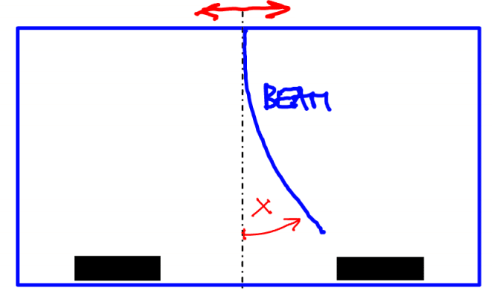
\includegraphics[width=0.5\textwidth]{figures/ch6/1forced_slender_beam.png}
		\caption{Depiction of the periodically forced slender beam. The frame is given by the blue rectangle. The two permanent magnets are represented by the black boxes.}
		\label{fig:forced_slender_beam}
	\end{figure}
This leads to the equation of motion
\begin{align}
	\ddot{x} + \dot{x} - x + x^3 = \varepsilon \cos(t);\quad 0 \leq \varepsilon \ll 1.
\end{align}
Therefore we have a perturbed Duffing oscillator. We transform the system into a first order ODE
\begin{align}
	\begin{dcases}
		\dot{x} = y \\
		\dot{y} = -y +x - x^3 + \varepsilon \cos(t).
	\end{dcases}
\end{align}
For $\varepsilon =0$ driving, two homoclinic orbits arise for the three fixed points. However, for nonzero driving, we get seemingly chaotic behavior. Both of these regimes are depicted in Fig. \ref{fig:pert_duffing}.
\begin{figure}[h!]
	\centering
	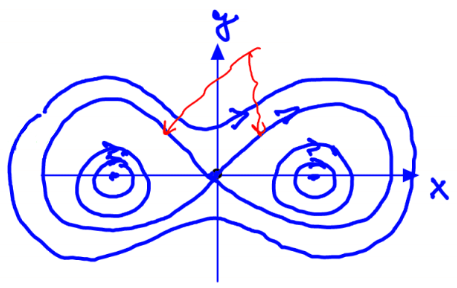
\includegraphics[width=0.45\textwidth]{figures/ch6/3unpert_duffing.png}
	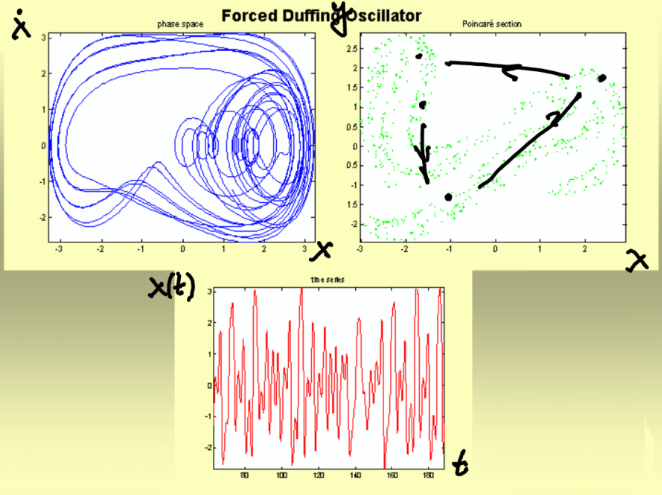
\includegraphics[width=0.45\textwidth]{figures/ch6/2pert_duffing.png}
	\caption{Left: Duffing oscillator with $\varepsilon=0$ driving, the red arrows designate the homoclinic orbits. Right: (Clockwise from top left) The phase space of the driven Duffing oscillator; The Poincaré section of the driven Duffing oscillator, with the Poincaré map illustrated by the black arrows; The value of $x(t)$ over time, with no apparent pattern.}
	\label{fig:pert_duffing}
\end{figure}

\end{ex}

\begin{ex}[2-dimensional Rayleigh-Bénard convection]
	A fluid is held between two plates. The upper plate is cold and the lower plate is hot. This causes convections to start as hotter fluid rises and colder fluid falls. So called convection cells then form for low Rayleigh numbers. This process is illustrated in Fig. \ref{fig:convection_cells}.
	\begin{figure}[h!]
		\centering
		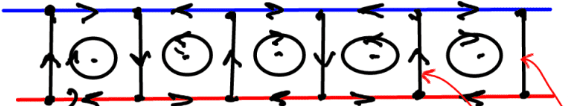
\includegraphics[width=0.65\textwidth]{figures/ch6/4convection_plates.png}
		\caption{Convection cells forming between two plates of different temperature. The cold plate (blue) is vertically above the hot plate (red). Each black dot represents a fixed point of the system, with heteroclinic orbits connecting them (red arrows). This is in an unperturbed setting ($\varepsilon =0 $).}
		\label{fig:convection_cells}
	\end{figure}

	If the Rayleigh number $R_{a}$ exceeds a critical value $R_{a_{ \textrm{crit} }}$, we have a time periodic perturbation to the velocity field. The fluid trajectories have the following equations of motion
	\begin{align}
		\begin{dcases}
			\dot{x} = u(x,y) + \varepsilon u_1(x,y,t) \\
			\dot{y} = v(x,y) + \varepsilon v_1 (x,y,t)
		\end{dcases}
;\quad \varepsilon>0.		
	\end{align}
	Here, the functions $u_1$ and $v_1$ are $T$-periodic. The chaotic nature of this system is shown in Fig. \ref{fig:convection_chaos}.
	\begin{figure}[h!]
		\centering
		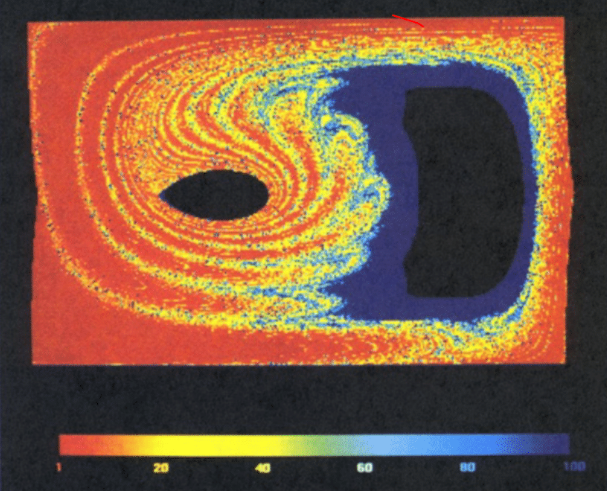
\includegraphics[width=0.4\textwidth]{figures/ch6/5convection_chaos.png}
		\caption{Escape time from one convection cell. The number of iterations of the Poincaré map needed for escape is given by the color scale. Here $0 < \varepsilon \leq 1$.}
		\label{fig:convection_chaos}
	\end{figure}
	
\end{ex}

Moving forward we will have a common mathematical setting
\begin{align}
	\dot{x} = f(x) + \varepsilon g(x,t);\quad x \in \mathbb{R}^{2},\quad g(x,t) =g(x,t+T);\quad 0 \leq \varepsilon \ll 1;\quad f,t\in \mathcal{C}^{1}. \numberthis \label{eq7:one}
\end{align}
We have a small $T$-periodic perturbation of a planar ODE which can be studied via a Poincaré map $P_{\varepsilon}^{t_0}:x_0 \mapsto x(t_0 + T; t_0,x_0)$. Assume that for $\varepsilon=0$ the system \eqref{eq7:one} has a saddle type fixed point with a homoclinic (or heteroclinic) orbit $x^{0}(t-t_0)$. Such a system is depicted in Fig. \ref{fig:assumptions}.
\begin{figure}[h!]
	\centering
	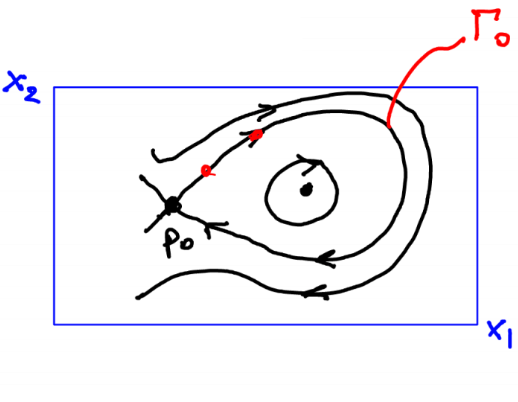
\includegraphics[width=0.45\textwidth]{figures/ch6/6assumptions_a.png}
	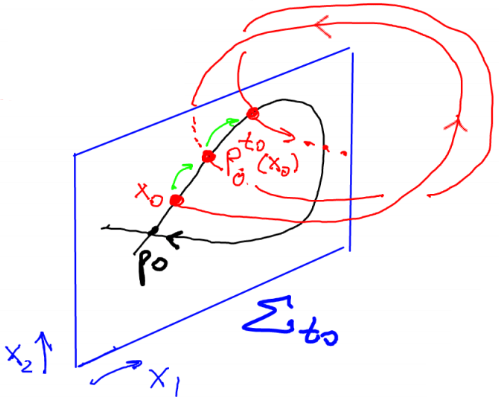
\includegraphics[width=0.45\textwidth]{figures/ch6/7assumptions_b.png}
	\caption{Left: An example of a system following the assumptions. The homoclinic orbit $\Gamma_0$ is equal to the local unstable and local stable manifolds. Right: The Poincaré map for $\varepsilon=0$, with time running counterclockwise about the $x_1$ axis with period $T$.}
	\label{fig:assumptions}
\end{figure}

\begin{remark}[]
	The fixed point of $P_{0}^{t_0}$ given by $p_0 $ is hyperbolic
	\begin{align}
	P_{0}^{t_0}(p_0) = p_0;\quad DP_{0}^{t_0}(p_0)  \textrm{ has eigenvalues }  \lambda_1,\lambda_2:\ |\lambda _1|<1,\ |\lambda _2|>1.
	\end{align}
	
\end{remark}

More generally we define a hyperbolic fixed point for a map.
\begin{definition}
	For a map $F:\mathbb{R}^{n}\to \mathbb{R}^{n}$ and a dynamical system with $x_{k+1} = F(x_k)$, the fixed point $p_0$ (i.e. $F(p_0) = p_0 $) is \emph{hyperbolic} if the linearization's $DF(p_0)\in \mathbb{R}^{n\times n}$ eigenvalues $\lambda_1,\ldots,\lambda_n $ never have unitary length: $|\lambda_i| \neq 1$ for $i=1,\ldots,n$.
\end{definition}

For each eigenvalue $\lambda _i$ of the linearization the corresponding eigenvector is given by $s_i$. Assume that $DF(p_0)$ is semisimple, i.e. all of the eigenvectors are linearly independent. The linearized dynamics at $p_0$ for $y=x-p_0$ small is 
\begin{align}
	y_{k+1} = DF(p_0)y_k \implies y_k = \lambda_1^{k} c_1 s_1 + \ldots + \lambda_n^{k} c_n s_n.	
\end{align}
If all of the eigenvalues have less than unitary magnitude, $|\lambda _i|<1$ for $i=1,\ldots,n$, then $p_0$ is asymptotically stable. Otherwise if there exists an eigenvalue with modulus strictly larger than 1, $p_0$ is unstable. The relationship of the nonlinear and linearized dynamics are shown in Fig. \ref{fig:lin_nonlin_relation}.
\begin{figure}[h!]
	\centering
	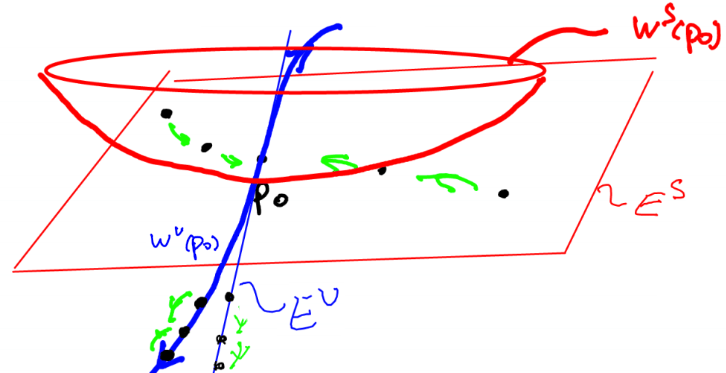
\includegraphics[width=0.65\textwidth]{figures/ch6/9lin_nonlin_relationship.png}
	\caption{The stable ($W^{S}(p_0)$) and unstable ($W^{U}(p_0)$) manifolds drawn in relation to the stable ($E^{S}$) and unstable ($E^{U}$) subspaces. The subspaces are given as the span of the stable (resp. unstable) eigenvectors. The green arrows signify steps of the linearized (resp. original) system.}
	\label{fig:lin_nonlin_relation}
\end{figure}

The fixed point $p_0$ along with the stable and unstable manifolds ($W^{S}(p_0)$ and $W^{U}(p_0)$) persist smoothly under small smooth perturbations to $F$ near $p_0$.

\section{Consequences of hyperbolicity}
Hyperbolicity has a few important consequences in our setting. Foremost, the perturbed hyperbolic fixed point $p_{\varepsilon}^{t_0}$ translates to a hyperbolic periodic orbit for the ODE. Furthermore, the solutions of the ODE are smooth in $\varepsilon$, thus the solutions within $W^{U}(p_{\varepsilon}^{t_0})$ and $W^{S}(p_{\varepsilon}^{t_0})$ remain $\mathcal{O}(\varepsilon)$ close to $\Gamma_0$, i.e.

\begin{subequations}
\begin{align}
	x_{\varepsilon}^{S}(t;t_0) &= x^{0}(t-t_0) + \varepsilon a^{S}(t) + \mathcal{O}(\varepsilon^{2} );\quad t\in [t_0,\infty ) \\
	x_{\varepsilon}^{U}(t;t_0) &= x^{0}(t-t_0) + \varepsilon a^{U}(t) + \mathcal{O}(\varepsilon^{2} );\quad t\in (-\infty, t_0].
\end{align}
\end{subequations}

Now we examine what the global shape of these manifolds are for $\varepsilon>0$ and if they interact. To do this we will follow an idea from Poincaré, Arnold, and Melnikov. To this end we define the perpendicular vector to $f$ 
\begin{align}
	f^{\perp}(x^{0}(0)) = 
	\begin{pmatrix}
		-f_2(x^{0}(0)) \\ f_1 (x^{0}(0))
	\end{pmatrix}
	.
\end{align}
We would like to use this to measure the distance between $x^{U}_{\varepsilon}(t_0;t_0)$ and $x^{S}_{\varepsilon}(t_0;t_0)$. The outlook for this is shown in Fig. \ref{fig:PAM_idea}.
\begin{figure}[h!]
	\centering
	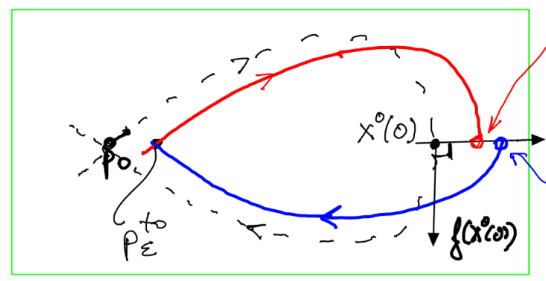
\includegraphics[width=0.5\textwidth]{figures/ch6/10PAM_idea.png}
	\caption{The Poincaré-Arnold-Melnikov idea. The dotted black line signifies $\Gamma$, the red dot $x^{U}_{\varepsilon}(t_0;t_0)$, the blue dot $x^{S}_{\varepsilon}(t_0;t_0)$, and the arrow pointing to the right $f^{\perp}$. The plane is $\Sigma_{t_0}$.}
	\label{fig:PAM_idea}
\end{figure}
Thus we have a signed distance function
\begin{align}
	d_{\varepsilon}(t_0) = \frac{\left\langle f^{\perp}(x^{0}(0)), x^{U}_{\varepsilon}(t_0; t_0) - x^{S}_{\varepsilon}(t_0; t_0)\right\rangle}{\left| f^{\perp}(x^{0}(0))\right|} 
	= \varepsilon  \frac{\left\langle f^{\perp}(x^{0}(0)), a^{U}(t_0) - a^{S}(t_0) \right\rangle}{\left| f^{\perp}(x^{0}(0))\right|} + \mathcal{O}(\varepsilon^2).
\end{align}
The numerator in the second equation is called the \emph{Melnikov function}
\begin{align}
	M(t_0)=\left\langle f^{\perp}(x^{0}(0)), a^{U}(t_0) - a^{S}(t_0) \right\rangle	.
\end{align}
In fact Melnikov proved an identity for this function.
\begin{theorem}[Melnikov]
	\begin{align}
		M(t_0) = \int_{-\infty }^{\infty }  \langle f^{\perp}(x^{0}(t-t_0)), g(x^{0}(t-t_0),t)\rangle dt.
	\end{align}
	For the proof, see \cite{GuckenheimerHolmes}.	
\end{theorem}
\begin{remark}[]
	The integral in Melnikov's theorem converges as $|g(x^{0}(t-t_0),t)|$ is globally bounded as $t \to \pm \infty $ and $|f^{\perp}| = |f|$ and
	\begin{align}
		\lim_{t\to \pm \infty }\left| f(x^{0}(t-t_0)) \right| =0,
	\end{align}
	exponentially as $p_0$ is a hyperbolic fixed point.	
\end{remark}

\begin{remark}[]
	In order to evaluate $M(t_0)$ we do not need to solve the perturbed ODE $\dot{x} =f(x) + \varepsilon g(x,t)$, instead we only need $x^{0}(t-t_0)$.
\end{remark}

Now observe that
\begin{align}
	d_{\varepsilon} (t_0) = 0 \iff \varepsilon \frac{M(t_0)}{\left| f^{\perp}(x^{0}(0))\right|} + \mathcal{O}(\varepsilon^2) = 0 \overset{\varepsilon \neq 0}{\iff} \underbrace{\frac{M(t_0)}{\left| f^{\perp}(x^{0}(0)) \right|} + \mathcal{O}(\varepsilon)=0}_{F(t_0, \varepsilon) = 0}.
\end{align}
Now we would like to know when we can find a solution $t_0(\varepsilon)$ such that $d_{\varepsilon}(t_0(\varepsilon))=0$ for $\varepsilon > 0$. To do this we use the Implicit Function Theorem. First assume that $F(\overline{t}_{0}, 0) = 0$, i.e. $M(\overline{t}_0) = 0$, and $\frac{\partial F}{\partial t_0}(\overline{t}_0), 0) \neq 0$, i.e. $\frac{\partial }{\partial t_0}M(\overline{t}_0) \neq 0$. If this condition is fulfilled the root is called \emph{transverse}.  Then there exists a unique $t_0(\varepsilon) = \overline{t}_{0} + \mathcal{O}(\varepsilon)$ which solves $F(t_0(\varepsilon), \varepsilon)=0$ for $\varepsilon \neq 0$ small enough. Also $t_0(\varepsilon)$ is smooth if $F(t_0,\cdot)$ is smooth.

A transverse zero for $M(t_0)$ implies that the Melnikov distance $d_{\varepsilon }(t_{0}(\varepsilon)=0$, in turn implying that the stable and unstable manifolds intersect, $W^{S}(p_{\varepsilon}^{t_0}) \cap W^{U}(p_{\varepsilon}^{t_0}) \neq \emptyset$. Therefore we have an element $q\in W^{S}(p_{\varepsilon}^{t_0}) \cap W^{U}(p_{\varepsilon}^{t_0})$, for this $q$ we also have that for every $n \in \mathbb{Z}$
\begin{align}
	P_{\varepsilon}^{n}(q) \in W^{S}(p_{\varepsilon}^{t_0}) \cap W^{U}(p_{\varepsilon}^{t_0}). 
\end{align}
Therefore we have that for each iterate of the Poincaré map there is a unique point in both the stable and unstable manifolds, so these must intersect each other infinitely many times. This behavior is shown in Fig. \ref{fig:inf_intersections}. 
\begin{figure}[h!]
	\centering
	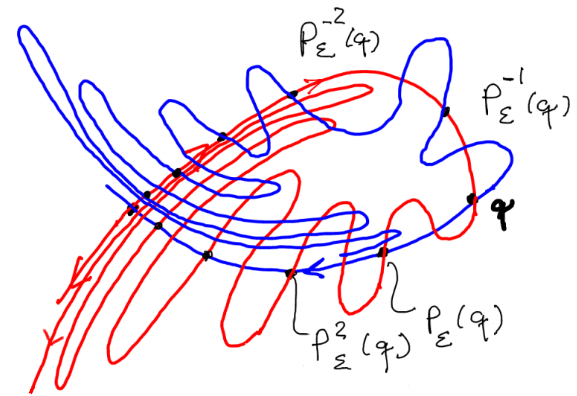
\includegraphics[width=0.45\textwidth]{figures/ch6/11inf_intersection_hetero.png}
	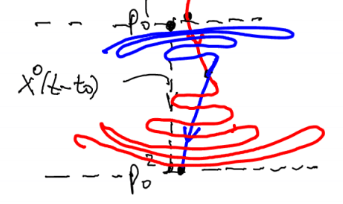
\includegraphics[width=0.45\textwidth]{figures/ch6/11inf_intersection_homo.png}
	\caption{The infinite intersections of the stable and unstable manifolds for a transverse zero. Left: The homoclinic case, this is aptly called a \emph{homoclinic tangle}. Right: The heteroclinic case.}
	\label{fig:inf_intersections}
\end{figure}
In the homoclinic tangle, we can see the accumulation of trajectories that are caused by the accumulation of the iterates of the Poincaré map. The accumulation can be formally seen as a consequence of the $\Lambda${\emph-lemma} \cite{PalisPhd, Palis}.

\begin{remark}[]
	It is impossible for stable and unstable manifolds to intersect themselves. This is usually argued by stating that $q$ cannot have two distinctive preimages under a diffeomorphism. However, this is not sufficient as a self intersection does not imply that two distinct preimages exist, for instance a looping manifold structure and suitable Poincaré map as in Fig. \ref{fig:loopdeloop}.
	\begin{figure}[h!]
		\centering
		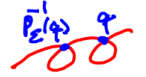
\includegraphics[width=0.25\textwidth]{figures/ch6/12loopdeloop.png}
		\caption{An example for a self-intersecting manifold without $q$ having multiple preimages.}
		\label{fig:loopdeloop}
	\end{figure}
A priori, this is possible to occur. In this case the existence of one loop actually implies the existence of infinitely many converging to $p_{\varepsilon}$. Thereby there must exist a loop in every arbitrarily small neighborhood of $p_{\varepsilon}$, this then contradicts the Hartman-Grobman Theorem as our system must be topologically equivalent to the linear saddle in a small enough neighborhood. 	
\end{remark}

\begin{remark}[]
	For every pair of intersections $P_{\varepsilon}^{k}(q)$ and $P _{\varepsilon}^{k+1}(q)$, there exists at least another intersection between the stable and unstable manifolds. This is due to the fact that $P_{\varepsilon}$ is orientation preserving (i.e. $DP_{\varepsilon}(q)$ is an orientation preserving linear map). The implication here is illustrated in Fig. \ref{fig:between_intersections}.
\begin{figure}[h!]
	\centering
	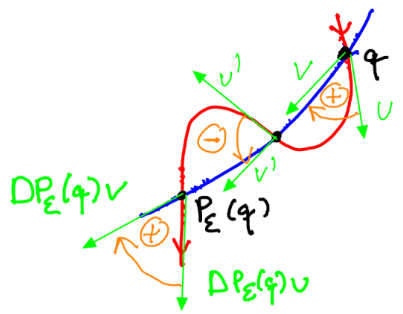
\includegraphics[width=0.5\textwidth]{figures/ch6/13between_intersections.png}
	\caption{Another intersection of the stable and unstable manifolds exists between two sequential iterates of the Poincaré map due to the preservation of orientation under this map.}
	\label{fig:between_intersections}
\end{figure}

The orientation preserving nature of $P_{\varepsilon}$ can be seen by using Liouville's Theorem. It states that for a general dynamical system $\dot{x}=f(x,t)$, the linearization of its flow-map $F_{t_0}^t:x_0 \mapsto x(t;t_0, x_0)$ satisfies 
	\begin{align}
		\det(DF_{t_0}^{t}(p)) = \exp \left( \int_{t_0}^{t}  \nabla \cdot ( f(x(s;t_0,p),s))ds\right).
	\end{align}
In our case we find
	\begin{align}
		\det (DP_{\varepsilon}(q)) = \exp\left(\int_{t_0}^{t_0+T} \nabla \cdot \left. (f + \varepsilon g) \right|_{x_{\varepsilon}(t);\ x_{\varepsilon}(t_0)=q}) ds \right) > 0
	\end{align}
	Therefore $DP_{\varepsilon}(q)$ is orientation preserving, in fact Poincaré maps in general are orientation preserving.	
\end{remark}

\begin{ex}[The forced-damped Duffing equation]
Recall the dynamical system
\begin{align}
	\begin{dcases}
		\dot{x}=y \\
		\dot{y} = x - x^3  + \varepsilon ( \gamma \cos(\omega t) -\delta y)
	\end{dcases}
	;\quad |\varepsilon|\ll 1.
\end{align}
Here the forcing amplitude is given by $\gamma $ and the linear damping coefficient by $\delta $. We separate the right hand side into two parts
\begin{align}
	f(x,y) = 
	\begin{pmatrix}
		y \\ x - x^3
	\end{pmatrix},\quad
	g(x,y) =
	\begin{pmatrix}
	0 \\  \gamma \cos(\omega t) -\delta y
	\end{pmatrix}
	. \numberthis \label{eq7:juan}
\end{align}
The Hamiltonian for the unperturbed system is given by
\begin{align}
	H = \frac{1}{2}y^2 - \frac{1}{2} x^2  + \frac{1}{4}x^4. %= E_{0} =  \textrm{const} .
\end{align}
Since the Hamiltonian is conserved, the trajectories of the unperturbed system are contained in the level sets of $H$. This allows us to draw the phase portrait that is shown in Fig. \ref{fig:duffing_phase}.
\begin{figure}[h!]
	\centering
	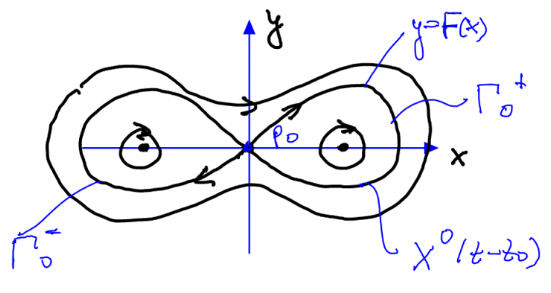
\includegraphics[width=0.5\textwidth]{figures/ch6/14duffing_phase.png}
	\caption{The phase portrait for the forced-damped Duffing oscillator for $\varepsilon=0.$}
	\label{fig:duffing_phase}
\end{figure}
The homoclinic orbit $\Gamma_0$ is contained in the $H=0$ level set of the Hamiltonian, which means that along this orbit we have
\begin{subequations}
\begin{align}
\frac{1}{2}y^2 -\frac{1}{2}x^2+\frac{1}{4}x^4 &=0. \\
\frac{dx}{dt}= y = \pm \sqrt{x^2-\frac{1}{2}x^2} &= F(x).
\end{align}
\end{subequations}

Locally we can obtain a parametrization of the heteroclinic orbit by solving this separable differential equation as
\begin{align}
	\frac{dx}{dt} = F(x) \implies \int_{0}^{x}  \frac{d \tilde{x}}{F(\tilde{x})} = \int_{0}^{t} d \tilde{t}.
\end{align}
Hence, on $\Gamma_{0}^{+}$, we have 
\begin{align}
	x^0(t) = 
	\begin{pmatrix}
		\sqrt{2}  \textrm{sech}(t) \\  -\sqrt{2}  \textrm{sech} (t) \tanh(t)
	\end{pmatrix}
.	
\end{align}
As discussed above, for $\varepsilon > 0$, the homoclinic orbit splits into a stable and an unstable manifold. We can now calculate the Melnikov function to study whether these manifolds intersect.
\begin{subequations}
\begin{align}
	M^{+}(t_0) &= \int_{-\infty }^{\infty }\langle f^{\perp}(x^{0}(t-t_0), g(x^{0}(t-t_0), t) \rangle dt \\
		   &= - \frac{4 \delta }{3} + \sqrt{2} \gamma \pi \omega  \textrm{sech} \left( \frac{\pi \omega }{2}\right)\sin(\omega t_0). 
\end{align}
\end{subequations}
Next, we ask if the Melnikov function is equal to zero. For an accumulation of intersection points, a homoclinic tangle, we also need a transverse zero. To this end we define $R^{0}(\omega) = \frac{4 \cosh \left( \frac{\pi \omega }{2}\right)}{3 \sqrt{2} \pi \omega }$. Thus the zeros of the Melnikov function are given by
 \begin{align}
	 R^{0}(\omega) = \frac{\gamma }{\delta} \sin(\omega t_0).
\end{align}
For a zero to exist, $R^{0}(\omega)$ cannot exceed the value $\frac{\gamma }{\delta}$, as $\sin(\omega t_0)$ is bounded by $1$. Therefore when we have $R^{0}(\omega) \leq \frac{\gamma }{\delta }$, a root of the Melnikov function exists. This root is non-transverse only when it is quadratic, i.e. when only a peak of the sine function intersects with $R^{0}(\omega) $. This occurs exactly when $R ^{0}(\omega)=\frac{\gamma }{\delta}$. In all other cases, the sine wave intersects the curve of $R^{0}(\omega) $ transversely, i.e. the zero is transverse. This is illustrated in Fig. \ref{fig:beam_tangle}, where equality occurs along the graph of $R^{0}$, that is the set on which non-transverse zeros exist. The area above this curve contains all of the point for which the zero is transverse.
\begin{figure}[h!]
	\centering
	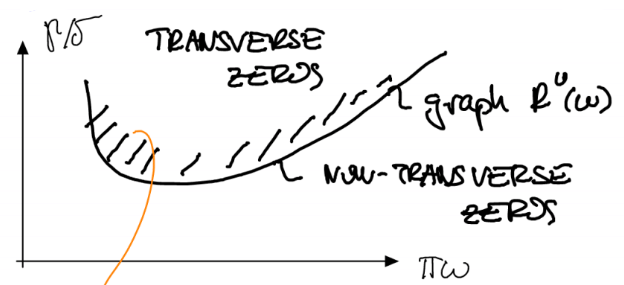
\includegraphics[width=0.6\textwidth]{figures/ch6/15beam_tangle.png}
	\caption{The yellow line designating the area above the curve where homoclinic tnagles exist for the forced-damped Duffing oscillator.}
	\label{fig:beam_tangle}
\end{figure}
\end{ex}

\section{Dynamics near the homoclinic tangle \& Smale's horseshoe map}
We now continue and examine the dynamics near the homoclinic tangle. Consider the dynamical system
\begin{align}
	\dot{x} = f(x) + \varepsilon g(x,t);\quad x \in \mathbb{R}^{2};\quad f,g \in  \mathcal{C}^{1};\quad g(x,t) = g(x,t+T).
\end{align}
With a linear change of coordinates we can  align our coordinate axes with the stable and unstable subspaces of the fixed point. Near the fixed point this leads to \emph{Smale's construction}, which is as shown as in Fig. \ref{fig:smales_construction}.
\begin{figure}[h!]
	\centering
	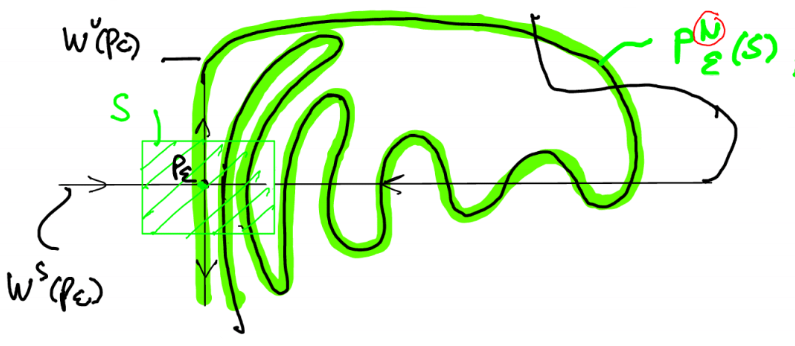
\includegraphics[width=0.7\textwidth]{figures/ch6/16smales_construction1.png}
	\hspace{0.03\textwidth}
	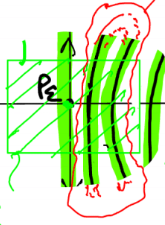
\includegraphics[width=0.25\textwidth]{figures/ch6/16smales_construction2.png}
	\caption{Smale's construction is found through an appropriate change of coordinates. Left: The full construction, the $N$ circled in red is large enough such that $P^{N}_{\varepsilon}(S)\cap S = \emptyset$, where $S$ is the green rectangle around $p_{\varepsilon}$. Right: Focus on the set $S$, the red lines designate a horseshoe-like structure.}
	\label{fig:smales_construction}
\end{figure}

A model for the right panel of Fig. \ref{fig:smales_construction} is given by \emph{Smale's horseshoe map}. This is defined by first considering the unit square $S=[0,1]^2\subset \mathbb{R}^{2}$, next the map itself is given by $f:S\to\mathbb{R}^{2}$. The map $f$ will not be defined explicitly, and instead geometrically. The unit square is divided into three horizontal strips, the upper one being labelled as $H_2$ and the lower $H_1$. The square is then squeezed horizontally and stretched vertically, and then smoothly bent to a horseshoe such that the previously upper horizontal strip now forms a vertical strip on the right side of the box $V_2$. Similarly, the lower horizontal strip now forms a vertical strip on the left $V_1$. Now the unit square can also be divided into three vertical strips, on the left $V_1$, an area in the middle, and on the right $V_2$. What was previously part of the middle horizontal strip is now mapped outside the unit square. Because the map is continuous, these points connect $V_1$ and $V_2$, but note that precisely defining what happens to these points is not essential in Smale's construction. The horseshoe map is depicted in Fig. \ref{fig:smale_map}. This is a good model for the dynamics near the homoclinic tangle, if we consider the horseshoe map $f$ to be many iterations of the Poincaré map $P^N_\varepsilon$ (for $N\gg 1$).
\begin{figure}[h!]
	\centering
	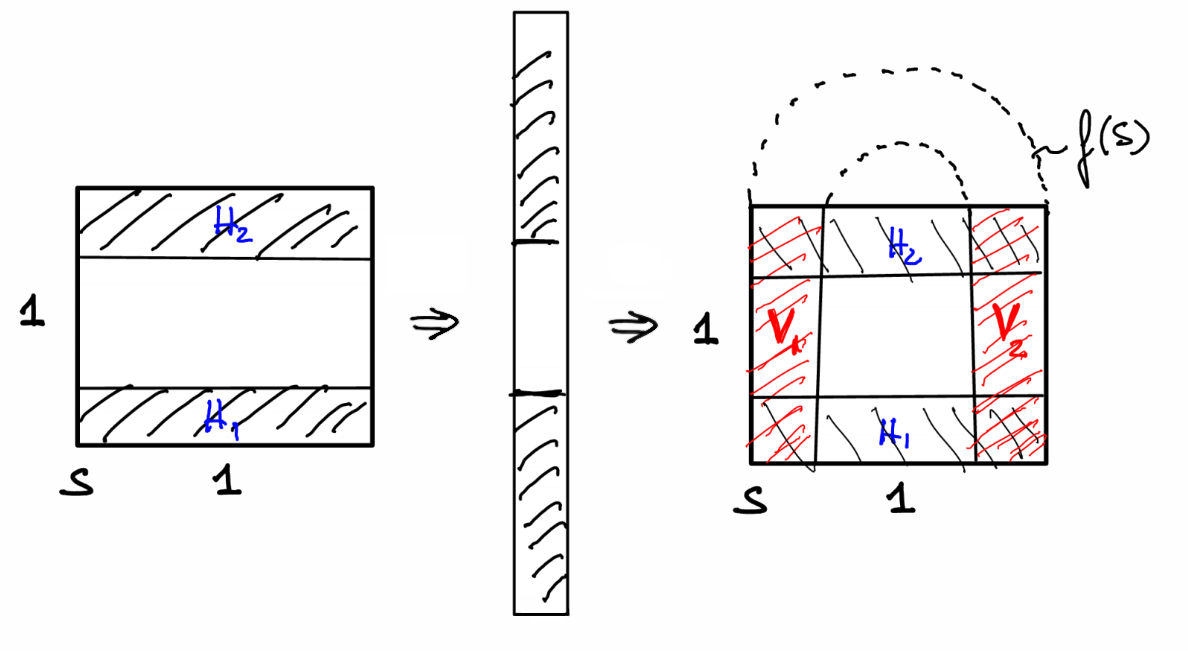
\includegraphics[width=0.8\textwidth]{figures/ch6/17smale_map.png}
	\caption{The two geometric steps of the Smale map, first a vertical stretch and then a fold into the horseshoe.}
	\label{fig:smale_map}
\end{figure}

Using this construction, we would like to know if any initial conditions stay in $S$ for long times (after many iterations of the horseshoe map), despite the overall instability coming from $P_{\varepsilon}$. To further study this we introduce a couple of definitions.
\begin{definition}
	The set of all points that stay in $S$ under $k$ backwards iterations is given by $V^{k}$.
\end{definition}
\begin{definition}[]
	For a map $f:X \to Y$, we denote the \emph{preimage} of a set $U\subset Y$ (or point $p\in Y$) as
	\begin{align}
		\boxed{
			f^{-1}(U) = \left\{ x\in X:\ f(x) \in U\right\}.
		}
	\end{align}
\end{definition}

The set of points that will be mapped into $S$ in one iteration is given by $S\cap f^{-1}(S)$. This means, that the set of points that stay in $S$ for one backward iteration, $V^1$, is
\begin{align}
V^1=f(S\cap f^{-1}(S)) = f(S)\cap f(f^{-1}(S)) = f(S)\cap S.
\end{align}
However, from the definition of the horseshoe map, $V^1 = f(S)\cap S$ is $V_1\cup V_2$, which is a closed, nonempty set. Similarly, for 2 backward iterations we have
\begin{align}
	V^{2} = f^{2}\left(S \cap f^{-1}(S) \cap f^{-2}(S) \right) = f^{2}(S) \cap f(S) \cap S  = V_{11} \cup V_{12} \cup V_{22} \cup V_{21} = \bigcup_{i_k \in \{1,2\}} V_{i_1i_2}.
\end{align}
The sets $V_{ij}$ are defined in Fig. \ref{fig:V_subsets}, the indices for each component are given by their orbit: The first index denotes which vertical strip $V_i\ (i\in \{1,2\})$ the preimage of a point is in. The second index denotes which vertical strip is it mapped into. That is, $V_{11}$ is the set of points that are mapped from $V_1$ to $V_1$ under one iteration, $V_{12}$ is the set of points mapped from $V_1$ to $V_2$ and so on. Also the set $V^{2}$ is closed, nonempty, contained in $V^{1}$, and has $2^2$ components.
\begin{figure}[h!]
	\centering
	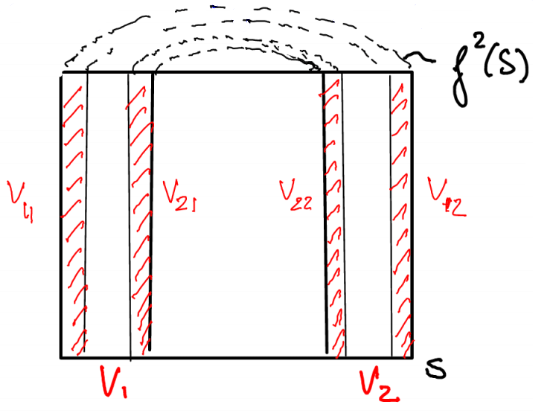
\includegraphics[width=0.35\textwidth]{figures/ch6/18V_subsets.png}
	\caption{The four components of $V^{2}$ with their index labels.}
	\label{fig:V_subsets}
\end{figure}

This continues for any number of backward iterates $k$ 
\begin{align}
	V^{k} = f^{k}\left(S \cap f^{-1}(S) \cap \ldots \cap f^{k}(S)\right) = f^{k}(S) \cap \ldots \cap f^{1}(S) \cap S = \bigcup_{i_j \in \{1,2\}}V_{i_1 \ldots i_k}.
\end{align}
This set has $2^k$ disjoint components (vertical strips) and is closed, nonempty, and contained in $V^{k-1}$. Therefore we have an infinite, nested sequence of nonempty and closed sets, therefore by Cantor's theorem we have 
\begin{align}
\boxed{
	V^{\infty } = \bigcap_{i=1}^{\infty } V^{i} \neq \emptyset.
}
\end{align}

\begin{remark}[]
	Cantor's theorem comes from the famous Cantor dust which arises by first removing the open middle third of the unit interval in $\mathbb{R}$, and then iteratively removing the open middle third of each remaining interval. The Cantor dust is a nonempty (in fact uncountably infinite) and disconnected set of points. For more on Cantor's theorem and Cantor's dust, see any book on measure theory.
\end{remark}

\begin{definition}
	A set $U$ is called \emph{perfect} if it is closed and has no isolated points, i.e. given any point $x\in U$ and any distance $\varepsilon$ we can find a distinct element $y\in U$ such that $\|x-y\| < \varepsilon$.
\end{definition}
\begin{remark}[]
	This definition uses that the topology on $U$ was induced by a metric, which may not be the case in general, but is not relevant to the content here.
\end{remark}

In our case $V^\infty$ is in fact a \emph{Cantor set of lines}, i.e. it is a closed, nonempty set which is totally disconnected (the largest connected component is a line), and perfect.
\begin{remark}[]
By a Cantor set of lines, we mean that there is a continuous, surjective map from this set of lines to a Cantor set of points. This map could be the one taking points along a vertical line to an intersection of the line with an arbitrarily selected horizontal line.
\end{remark}

\begin{definition}
	Analogous to before we define the set of all points that stay in $S$ under $k$ forwards iterations as $H^{k}$. For each $k$ the set $H ^{k}$ is a nonempty set of $2^k$ closed, disjoint, horizontal strips, forming a nested sequence.
\end{definition}
By similar reasoning as before we have 
\begin{align}
	\boxed{
		H^{\infty } = \bigcap_{k=1}^{\infty} H^{k} \neq \emptyset.
	}
\end{align}

\begin{definition}
	The set of all points that stay in $S$ for all forward and backward iterates of the Smale horseshoe map  is given by
	 \begin{align}
		\boxed{
\Lambda = H^{\infty } \cap V^{\infty }.
		}
	\end{align}
	The geometry of this set is shown in Fig. \ref{fig:lambda_def}.
	\begin{figure}[h!]
		\centering
		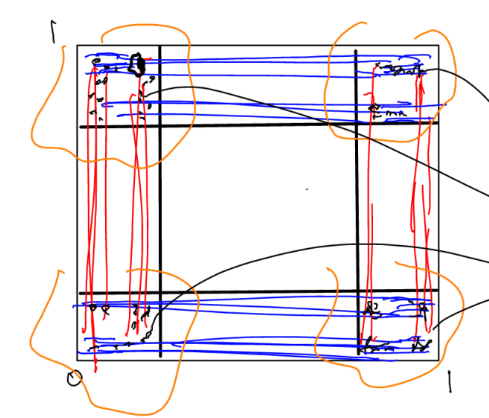
\includegraphics[width=0.4\textwidth]{figures/ch6/19lambda_def.png}
		\caption{The geometry of the set $\Lambda$, with the four regions containing points circled in orange. The red vertical lines represent the set $V^{\infty }$ and the blue horizontal lines the set $H^{\infty }$.}
		\label{fig:lambda_def}
	\end{figure}
\end{definition}

\begin{remark}[]
The set $\Lambda$ is a Cantor set of points.
\end{remark}

We have then identified the invariant set $\Lambda$ for the horseshoe map. Returning to our case study of a Poincaré map with a homoclinic tangle, the points in $\Lambda$ keep coming back forever to the unstable periodic orbit as shown in Fig. \ref{fig:returning_points}. 
\begin{figure}[h!]
	\centering
	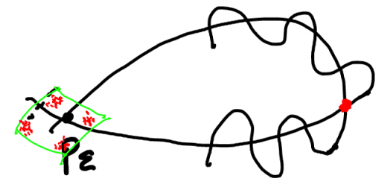
\includegraphics[width=0.3\textwidth]{figures/ch6/20returning_points.png}
	\caption{The homoclinic tangle with the set $S$ outlined in green and the elements of $\Lambda$ being denoted by the red dots within $S$.}
	\label{fig:returning_points}
\end{figure}

\section{Dynamics of Smale's horseshoe map on the invariant set $\Lambda$}
We label any point $p\in \Lambda$ with an infinitely long binary sequence, which reflects the itinerary of $p$ in $\Lambda$ under iterations of $f$. For a given $p$, if we have 
\begin{align}
	\ldots,\
	f^{-2}(p) \in V_{s_{-3}},\
	f^{-1}(p) \in V_{s_{-2}},\
	p \in V_{s_{-1}},\
	p \in H_{s_{0}},\
	f^{}(p) \in H_{s_{1}},\
	f^{2}(p) \in H_{s_{2}},\
\ldots	
\end{align}
for $s_i\in \{1,2\}$ then we would have the itinerary 
\begin{align}
	\boxed{
s  = \ldots s_{-3}s_{-2}s_{-1} \bm{.}  s_0 s_{1}s_{2}\ldots.
	}
\end{align}
This is a unique symbolic encoding for \underline{all} points in $\Lambda$. Therefore there is a one-to-one correspondence between points $p$ in the invariant set $\Lambda$ and sequences $s$ space of doubly infinite sequences of two symbols $\Sigma$. Such a space is just the space of outcomes for an infinite coin-tossing experiment. This equivalence of $\Lambda$ to the doubly infinite sequence of two symbols leads us to \emph{symbolic dynamics}: the analogue of the horseshoe map on the symbol space $\Sigma$.

In order to study these symbolic dynamics we need to know what the symbolic encoding of $f(p)$ is. For the analogue $\ldots s_{-2}s_{-1}\bm{.} s_0 s_1 s_2 \ldots = s\in \Sigma$ of $p\in \Lambda $, we can read off that $f(p)\in H_{s_1}$. Continuing in this fashion, we can see that $f(f(p))=f^{2}(p) \in H_{s_2}$ and so on, therefore $f(p)\in H^{\infty }$. By recalling that $f(H_{s_0}) = V_{s_0}$ we can see that $f(p) \in V_{s_0}$. Applying the definition of $f$ we find that $f^{-1}(f(p)) = p \in V_{s_{-1}}$. Therefore $f(p)\in V^{\infty }$ and thereby $f(p) \in \Lambda$. 

From our examination of the forward iterates of $f(p)$ we know that the symbolic encoding of $f(p)$ to the right of the dot is
\begin{align}
	\bm{.}s_1 s_2 s_3\ldots. 
\end{align}
Similarly, from our examination of the backwards iterates of $f(p)$ we know that the symbolic encoded of $f(p)$ to the left of the dot is
\begin{align}
\ldots s_{-2} s_{-1} s_{0} \bm{.}. 
\end{align}
Putting these together we get the symbolic encoding for $f(p)$ is 
\begin{align}
	\ldots s_{-2} s_{-1} s_{0} \bm{.} s_1 s_2 s_3 \ldots \in \Sigma.
\end{align}
So the encoding of $f(p)$ in the symbolic space is just a shift to the left on the encoding of $p$.

\begin{definition}
	We define the following three maps:
	\begin{enumerate}
		
\item The \emph{symbolic encoding map}
	\begin{align}
		\boxed{
			\phi:\Lambda \to \Sigma;\quad p \mapsto s= \phi(p);
		}
	\end{align}
This map can be shown to be a homeomorphism, i.e. it is continuous and has a continuous inverse. For a proof we refer to \cite{GuckenheimerHolmes}.

\item The \emph{Smale horseshoe map restricted to $\Lambda$}
	\begin{align}
		\boxed{
			\tilde{f}:\Lambda \to \Lambda;\quad p \mapsto f(p);
		}
	\end{align}
\item The \emph{Bernoulli shift map}
	\begin{align}
		\boxed{
			\sigma:\Sigma \to \Sigma;\quad
			\ldots s_{-2} s_{-1} \bm{.} s_0 s_1 s_2 \ldots 
			\mapsto
			\ldots s_{-2}s_{-1}s_{0}\bm{.} s_1 s_2 s_3 \ldots.
		}
	\end{align}
	
	\end{enumerate}
\end{definition}
We have that the following diagram commutes
\begin{equation}
\begin{tikzcd}
	\Sigma \arrow[r, "\sigma"] 
& \Sigma \\
\Lambda \arrow[u,"\phi"] \arrow[r, "\tilde{f}"]
& \Lambda \arrow[u, "\phi"] 
\end{tikzcd}.
\end{equation}
Therefore $\tilde{f} = \left. f\right|_{\Lambda}$ is topologically conjugate to a Bernoulli shift on $\Sigma$ 
	\begin{align}
		\tilde{f} = \phi^{-1} \circ \sigma \circ \phi.
	\end{align}
Hence, orbits of $f$ are taken to those of $\sigma$, with their orientation preserved.	

\begin{remark}[]
	To denote an infintely repeating string, the bar notation will be used i.e.
	\begin{align}
		\overline{1} = 111\ldots,\quad \overline{123}=123123\ldots.
	\end{align}
\end{remark}

It is possible to classify all of the orbits of $\sigma $ in $\Sigma$, the classes and their cardinality are as follows:
\begin{enumerate}
	\item \textbf{Fixed points} There are exactly two fixed points of $\sigma$, namely $\overline{1}\bm{.} \overline{1}$ and $\overline{2}\bm{.} \overline{2}$; 
	\item \textbf{Period-two orbits} A single such orbit exists, that of $\overline{12}\bm{.} \overline{12}$, as $\sigma^{2}(\overline{12}\bm{.} \overline{12}) = \sigma(\overline{21}\bm{.} \overline{21} = \overline{12}\bm{.} \overline{12}$;
	\item \textbf{Period-three orbits} There exists two such orbits, namely $\overline{112}\bm{.} \overline{112} \to \overline{121}\bm{.} \overline{121} \to \overline{211}\bm{.} \overline{211}$ and $\overline{221} \bm{.} \overline{221} \to \overline{212}\bm{.} \overline{212} \to \overline{122}\bm{.} \overline{122} $.
	\item \textbf{Period-$\bm{k} $ orbits} For every natural number $k$, there exists 
		\begin{align}
			\boxed{N(k) = \frac{1}{k}\left(2^k - \sum_{\langle i,k \rangle }^{} i N(i)\right)}		
		\end{align}
		orbits of period exactly $k$, the notation $\langle i,k\rangle$ signifies integers $i$ which are divisors of $k$.	
\end{enumerate}
There exists a countable infinity (i.e. the elements can be organized uniquely into an infinite countable sequence) of periodic orbits of arbitrarily high period. The countable sequence ordering can be done by listing each orbit in the row corresponding to its minimal period. An orbit of period $k$  is made up of $k$ points along that orbit. We assign a single number to the orbit by concatenating the decimal representations of the individual points along the orbit, starting from the one with the smallest value. Within a row, we can then order the periodic orbits based on the magnitudes of the concatenated numbers representing them. Thus $\overline{112}\bm{.} \overline{112}$ would go in the third row as it has the minimal period $3$, as the fixed points have period length $0$ and occupy the first row), and in the leftmost position as $\overline{112} \prec \overline{122}$. Each row has a finite number of elements, so ordering each row is not a problem. Then the complete order is done by starting with $0$ for the first element in the first row (the fixed point $\overline{1}\bm{.} \overline{1}$), then reading from left to right before continuing to the next row. This list is well defined and countably infinite, containing all of the orbits of $\sigma$.

Before further study, it is important to introduce a notion of distance on the space $\Sigma$.
\begin{definition}
	The distance on the space $\Sigma$ between two elements $s$ and $s'$ is given by
	\begin{align}
		d(s,s') = \sum_{i=-\infty }^{\infty } \frac{|s_i - s'_i |}{2^{|i|}}.
	\end{align}
Therefore two symbols are close if they agree on large central blocks.	
\end{definition}
\begin{remark}[]
	The function $d$ satisfies all the axioms of a distance and the tuple $(\Sigma, d) $ forms a complete metric space. 
\end{remark}

\begin{proposition}[The periodic orbits are dense]
The set of all periodic orbits is dense in $\Sigma$.	
\end{proposition}
%\begin{proof}
%	Given an arbitrary element $s\in\Sigma$ and $k \in \mathbb{N}$, we would like to find a $2^{-k}$ periodic approximation of $s$. To do this define the two strings
%	\begin{align}
%		S_{-} = s_{-(k+1)}\ldots s_{-1}, \quad S_{+} = s_0 \ldots s_{k+1}.
%	\end{align}
%	For any two strings (of infinite length) $L$ and $R$ the element
%	 \begin{align}
%		s' = L S_{-}\bm{.} S_{+}R
%	\end{align}
%	is $2^{-k}$ close to $s$. This is because they can only disagree at indices with modulus strictly greater than $k+1$, therefore
%	\begin{align}
%		d(s',s) \leq \sum_{j=-(k+2)}^{-\infty }\frac{1}{2^{-|j|}} + \sum_{j=k+2}^{\infty } \frac{1}{2^{-|j|}} = 2\cdot 2^{-(k+1)} = 2^{-k}. 
%	\end{align}
%Now it is clear that the periodic element
%\begin{align}
%	s^{*} = \overline{S_{+}S_{-}} \bm{.} \overline{S_{+}S_{-}} = L' S_{-}\bm{.} S_{+}R'
%\end{align}
%is a $2^{-k}$ approximation for $s$. As $s$ and $k$ were arbitrary, this completes the proof.
%\end{proof}
\begin{proposition}[]
Consider a $k$-periodic point $s=\overline{a}\bm{.} \overline{a}$, where $a$ is a $k$-long binary sequence. Let $s' = \overline{a}a'\bm{.} \overline{a}$, clearly $s \neq s'$, therefore $d(s,s') \neq 0$, when we take the limit we find
\begin{align}
	\lim_{n\to \pm \infty }	d(\sigma^{n}(s), \sigma^{n}(s')) = 0.
\end{align}
\end{proposition}


Thus the underlying periodic orbit is unstable. Furthermore, $s$ has a countable infinity of homoclinic orbits. As the periodic orbit was arbitrary, these statements hold for all periodic orbits, hence all periodic orbits are unstable and have a countable infinity of homoclinic orbits.

\begin{remark}[]
Also note that any two periodic orbits (of arbitrary period) are connected by a countable infinity of heteroclinic orbits.
\end{remark}
Together, there exists a countable infinity of periodic and asymptotically periodic orbits, a sketch of this behavior is shown in Fig. \ref{fig:crazy_orbits}.
\begin{definition}
	A point $s$ is asymptotically periodic if there is a periodic orbit $p$ such that 
	\begin{align}
		\boxed{
			\lim_{n\to \infty } d(\sigma^{n}(s), \sigma^{n}(p))=0.
		}
	\end{align}
For example, heteroclinic orbits are asymptotically periodic.
\end{definition}

\begin{figure}[h!]
	\centering
	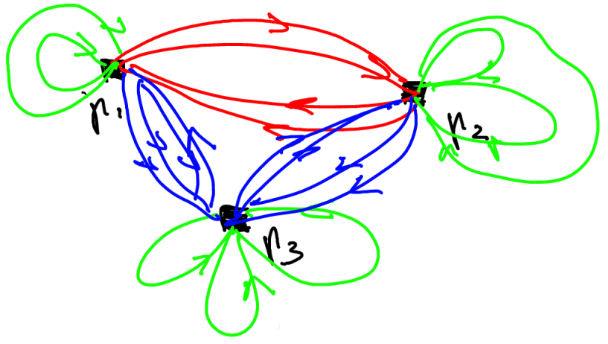
\includegraphics[width=0.55\textwidth]{figures/ch6/21crazy_orbits.png}
	\caption{A depiction of the (infinitely many) homo- and heteroclinic orbits which connect periodic orbits of $\sigma $.}
	\label{fig:crazy_orbits}
\end{figure}

In fact there also exists a countable infinity of non-periodic (not even asymptotically periodic) orbits in $\Sigma$. To show this, we will show that $\Sigma$ is uncountable, i.e. that it cannot be arranged into a well-defined, countable sequence.
\begin{definition}
	The binary expansion of a number $x\in [0,1]$ is the sequence $(b_i)_{i=1}^{\infty }$ of 1s and 0s  such that 
	\begin{align}
		x = \sum_{i=1}^{\infty } \frac{b_i}{2^i}.
	\end{align}
	To calculate this sequence define the map $g(x) = 2x \mod 1$. Then generate the sequence $(x_i)_{i=1}^{\infty }=(x, g(x), g^2(x), \ldots)$. Finally, set each binary coefficient as
	 \begin{align}
		b_i =
		\begin{cases}
			0 & 2x_i < 1 \\
			1 & 2x_i \geq 1
		\end{cases}.
	\end{align}
	
\end{definition}
\begin{proposition}[]
	The set $\Sigma$ is uncountable.
\end{proposition}
\begin{proof}
	It is enough to show that the set $\tilde{\Sigma}$ defined by 
	 \begin{align}
		 \tilde{\Sigma} = \{ \bm{.} s_1s_2s_3 \ldots:\ s_i\in \{0,1\}\}
	\end{align}
	is uncountable. This suffices as we can injectively embed $\tilde{\Sigma}$ into $\Sigma$ via the map $\bm{.} s_1s_2\ldots \mapsto \overline{1}\bm{.} (s_1+1)(s_2+1)\ldots$.

	Every binary expansion for all real numbers in the interval $[0,1]$ is contained within $\tilde{\Sigma}$, therefore the cardinality of $\tilde{\Sigma}$ is at least as large as that of $[0,1]$ which is uncountable. In fact, the binary expansion is a bijection, and these two sets have the exact same cardinality. 
\end{proof}

\begin{ex}[Binary expansion]
	Let $x=\frac{1}{5}$, we find the iterates of $g$ 
	\begin{subequations}
	\begin{align}
		x &= \frac{1}{5} & 2\cdot \frac{1}{5}<1 & \implies x_1 = 0\\
		g\left(\frac{1}{5}\right) &= \frac{2}{5} & 2 \cdot \frac{2}{5}<1 &\implies x_2 = 0 \\
		g^{2}\left(\frac{1}{5}\right) &= g\left(\frac{2}{5}\right) = \frac{4}{5} & 2\cdot \frac{4}{5} > 1 &\implies x_3 = 1 \\
		g^{3}\left(\frac{1}{5}\right) &= g\left(\frac{4}{5}\right) = \frac{8}{5} \mod 1 = \frac{3}{5}& 2\cdot \frac{3}{5} > 1	  &\implies x_4 = 1 \\
		g^{4}\left(\frac{1}{5}\right) &= g\left(\frac{3}{5}\right) = \frac{6}{5} \mod 1 = \frac{1}{5}& 2\cdot \frac{1}{5} < 1	  &\implies x_5 = 0. 
	\end{align}
\end{subequations}
	Since $g^{4}\left(\frac{1}{5}\right) = \frac{1}{5}$, we have reached a repeating loop (since our seed value was $\frac{1}{5}$), therefore we have that
	\begin{align}
		\frac{1}{5} = 0\cdot \frac{1}{2} + 0\cdot \frac{1}{4} + 1\cdot \frac{1}{8} + 1\cdot \frac{1}{16} + \ldots = \bm{.} \overline{0011}. 
	\end{align}
	
\end{ex}

\begin{remark}[]
	Recall that for a metric space $(X,d)$ when we write $\mathcal{B}\left(x, r\right) $ we refer to the open ball of radius $r $ around $x $, i.e.
	\begin{align}
		\mathcal{B}\left(x,r\right) = \left\{ y\in X:\ d(x,y) < r \right\}.
	\end{align}
\end{remark}

\begin{proposition}[]
	The map $\sigma$ has a dense orbit in $\Sigma$, i.e. an orbit which approaches any point in $\Sigma$ arbitrarily closely.
\end{proposition}
%\begin{proof}
%Without loss of generality, assume that $\delta<1$. Next, note that the maximal distance between two elements occurs when they disagree at every entry, so they have the distance
%\begin{align}
%	\sum_{i=-\infty }^{\infty } \frac{1}{2^{|i|}} = 2.
%\end{align}
%Therefore, the entire space is included in the ball $\mathcal{B}\left( \overline{1}\bm{.} \overline{1}, 2\right)$. Now to show that for any given distance $\delta $, we want to find an element $s^{*}$ such that its orbit gets $\delta$ close to every element of $\Sigma$. Let 
%\begin{align}
%k = \min \left\{ j \in \mathbb{N}:\ 2^{-j}\leq \delta\right\},
%\end{align}
%i.e. the first index in the binary expansion of $\delta$ which is not $0$. Now we would like to find a finite $2^{-(k+1)}$-covering of $\Sigma$, i.e. a set of elements $s_i^{k}$ such that $\bigcup_{i}\mathcal{B}\left(s_i^{k}, 2^{-(k+1)}\right)$. We start out with the covering $\bigcup_{j=1}^{\infty }\mathcal{B}\left(q_j, 2^{-(k+1)}\right)$, with the $q_j$ being an enumeration of the periodic orbits. As we previously noted, $\Sigma$ is bounded as it can be contained in a finite ball, furthermore $\Sigma$ is also closed (the intersection of two closed sets is always closed due to the de Morgan identity), thus $\Sigma$ is compact and a finite subcovering exists. Hence we can deduce that only finitely many $q_i$ are needed, call these $\left(s_i^{k}\right)_{i=1}^{N}$, and let the string representation of each $s_{i}^{k}$ be given by $\overline{S_{i}^{k}}\bm{.} \overline{S_{i}^{k}}$. 
%
%If we can construct $s_{k}^{*}$ such that its orbit passes through each of the $\mathcal{B}\left(s_i^{k}, 2^{-(k+1)}\right)$, then we know that the orbit of $s_{k}^{*}$ gets within distance $2^{-k}$ of every element in $\Sigma$, by the triangle inequality. 
%
%For any given $s_{i}^{k}$ the element
%\begin{align}
%	{L} \underbrace{S_{i}^{k} \ldots S_{i}^{k}}_{(k+3) \textrm{ times} }\bm{.}  \underbrace{S_{i}^{k} \ldots S_{i}^{k}}_{(k+4) \textrm{ times} } {R}
%\end{align}
%is within distance $2^{-(k+1)}$ of $s_{i}^{k}$, for $L$ and $R$ arbirary. This is because the string $S_{i}^{k}$ is of at least length 1, so the two strings can disagree only at elements with index modulus strictly greater than $k+2$ (we need the one more copy of $S_{i}^{k}$ on the right side as the 0th index is to the right of the $\bm{.} $ ), therefore the distance between them is upper bounded by
%	\begin{align}
%		\sum_{j=-(k+3)}^{-\infty }\frac{1}{2^{-|j|}} + \sum_{j = k+3}^{\infty } \frac{1}{2^{-|j|}} = 2 \cdot 2^{-(k+2)} = 2^{-(k+1)}.   	
%	\end{align}
%	Therefore, using $2k+7$ copies of $S_{i}^{k}$ we are able to approximate $s_{i}^{k}$ within distance $2^{-(k+1)}$. We now construct the element
%	\begin{align}
%		s_{k}^{*} = L \bm{.} \underbrace{S_{1}^{k} \ldots S_{1}^{k}}_{2k+7  \textrm{ times} } \ldots \underbrace{S_{N}^{k} \ldots S_{N}^{k}}_{2k+7  \textrm{ times} } R
%	\end{align}
%	for $L$ and $R$ arbitray. We now can see that for every $i\in\{1 \ldots N\}$, the element 
%	\begin{align}
%		L' \underbrace{S_{i}^{k} \ldots S_{i}^{k}}_{(k+3) \textrm{ times} } \bm{.} 
%		\underbrace{S_{i}^{k} \ldots S_{i}^{k}}_{(k+4) \textrm{ times} } R',
%	\end{align}
%	is contained within the orbit of $s_{k}^{*}$ for $L'$ and $R'$ chosen accordingly. Therefore we have now constructed the the desired $s_{k}^{*}$. Note here that this construction is well defined as each $S_{i}^{k}$ is of finite length. This construction can be done for each $k$: start from the infinite cover using periodic orbits, then construct a finite subcover using the compactness of $\Sigma$, finally construct the element $s_{k}^{*}$ by concatenating the $2^{-(k+1)}$ approximations of the elements which consitute the finite subcover. 
%
%	To construct $s^{*}$, concatenate each of the strictly defined blocks (the block the the right of $\bm{.} $ and left $R$) of $s_{k}^{*}$ for each $k \in \mathbb{N}$. For any $n$, we know that we can get within distance $2^{-n}$ distance of each element in $\Sigma$, therefore we have constructed a dense orbit. This construction is well definied as the strictly defined block of any given $s_{k}^{*}$ is always of finite length. Thus we have constructed the element, whose orbit is dense in $\Sigma$.
%\end{proof}

\begin{proposition}[]
	The map $\sigma$ is topologically transitive, i.e. for any two open sets $A$ and $B$ in $\Sigma$, there exists an $N \in \mathbb{N}$ such that
	\begin{align}
		\sigma^{N}(A) \cap B \neq \emptyset.
	\end{align}
\end{proposition}
	This is also called the \emph{mixing property}. In the case of the Bernoulli shift map, it can be concluded from the existence of a dense orbit.
\begin{proposition}[Sensitive dependece on initial conditions]
	Regardless of how close two distinct initial conditions $s$ and $s'$ are chosen, they will not remain close. There exists a $\Delta>0$ such that for every $s\in\Sigma$ and any $\delta>0$, there exists an $s' \in \mathcal{B}\left(s, \delta\right)$ such that for an $N$ large enough the following holds
	\begin{align}
		d(\sigma^{N}(s), \sigma^{N}(s') ) > \Delta.
	\end{align}
	This is called the \emph{uniform instability of all orbits}. This fact is depicted in Fig. \ref{fig:unif_instab}.	
\end{proposition}

\begin{figure}[h!]
	\centering
	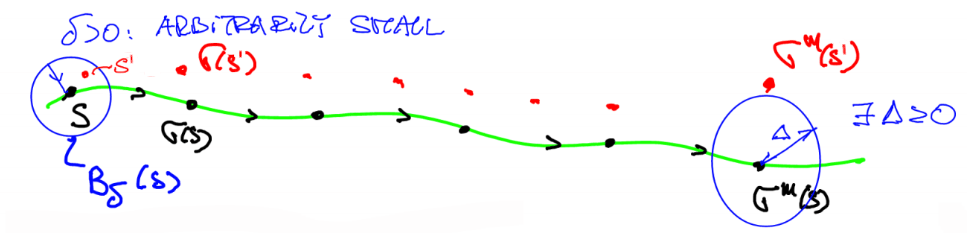
\includegraphics[width=0.8\textwidth]{figures/ch6/22unif_instab.png}
	\caption{The uniform instability of orbits for the map $\sigma$.}
	\label{fig:unif_instab}
\end{figure}

\begin{remark}[]
	This by itself implies no complexity: the linear saddle
	\begin{align}
		\begin{dcases}
			\dot{x} = \lambda x \\
			\dot{y} = - \mu y,
		\end{dcases}
	\end{align}
also has this property.	
\end{remark}

\begin{remark}[]
	In the case of this map, every $s'\in \mathcal{B}\left(s, \delta \right)$ has an $N$ large enough such that the inequality holds.
\end{remark}

These observations lead us to the following definition of a chaotic map.

\begin{definition}[Chaotic map]
	Let $M:C\to C$ be a $\mathcal{C}^{0}$ map on a compact metric space $C$. We call $M$ \emph{chaotic} if
	\begin{enumerate}
		\item $M$ is topologially transitive (the mixing property);
		\item $M$ has sensitive dependence on initial conditions (a lack of reproducibility);
		\item $M$ has a dense set of periodic orbits in $C$.
	\end{enumerate}
\end{definition}
The Bernoulli shift map $\sigma$ is chaotic, therefore Smale's horseshoe map on the invariant set $\Lambda$ is chaotic, therefore the horseshoe map on the unit square is chaotic. Since that was a model for the Poincaré map with a homoclinic tangle, we can rigorously conclude that the forced Duffing equation is chaotic. All this followed from a transverse zero of the Melnikov function.
 \begin{ex}[Chaos in a 1-dimensional model]
 	Consider the logistic map for resource-limited discrete population growth dynamics
	\begin{align}
		x_{n+1}=x_{n}= ax_n(1-x_n);\quad a \in \mathbb{R}^{+}.
	\end{align}
	We will now continue with $a=4$. The points $x=0$ and $x=\frac{3}{4}$ are fixed points. These are each unstable as $|f'(x)|>1$ at both of these points. This is not an ODE, and we do not assume that the model is a small perturbation of a simpler system. That is, we are not assuming persistence of known structures. The cobweb diagram is illustrated in Fig. \ref{fig:logistic_cobweb}.
	\begin{figure}[h!]
		\centering
		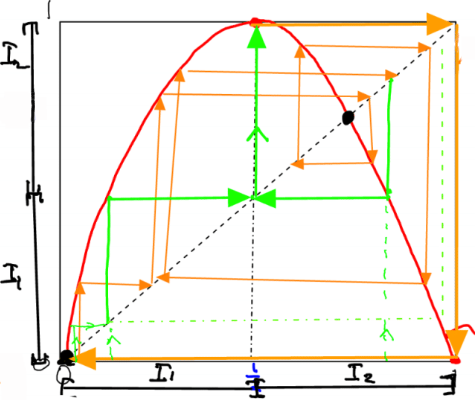
\includegraphics[width=0.4\textwidth]{figures/ch6/23logisitic_cobweb.png}
		\caption{The cobweb diagram for the logisitic map with $a=4$. The sets $I_1$ and $I_2$ are defined as $[0, \frac{1}{2}]$ and $[\frac{1}{2}, 1]$.}
		\label{fig:logistic_cobweb}
	\end{figure}
	We can see that for our choice of $a$, $f$ maps $[0,1]$ to $[0,1]$ and is not invertible. In fact each preimage of $\frac{1}{2}$ reaches $0$ in a finite number of iterations. Also note that because the map is quadratic, each point has two preimages. Following a point in backward time is not well defined in the usual sense, but instead, we may take preimages of preimages of $\frac{1}{2}$. This gives rise to two branches of backward iterates, i.e. two chains of preimages of $\frac{1}{2}$. One of these branches (branch A) converges to 0, and the other one (branch B) converges to $\frac{3}{4}$ in backward time. Points on branch A thus form a homoclinic orbit to zero, and points on branch B form a heteroclinc orbit between $\frac{3}{4}$ and $0$. Since a point may follow branch A for a finite number of backward iterations before switching to branch B and vice versa, we actually have a countably infinite number of homo- and heteroclinic orbits. From Fig. \ref{fig:logistic_cobweb}, the dynamics appears complicated, with no stable fixed points as we have seen from the linearization.

To better understand the dynamics we can encode the itinerary of a point $x\in I=[0,1]$ by if $x$ is in $I_{1}$ or $I_{2}$. We get a one-sided itinerary, because $f$ is not invertible. For example if $x\in I_{s_0}$, $f(x)\in I_{s_1}$, $f^{2}(x)\in I_{s_2}$ then we would encode $x$ as $\bm{.} s_0s_1s_2\ldots$ for $s_i \in \{ 1,2\}$.

Note here that this symbolic encoding is not well defined for every point in $I$, as all preimages of $x=\frac{1}{2}$ have multiple encodings, since their iterates eventually reach $I_{1}\cap I_{2} =\frac{1}{2}$. To address this, instead we hope to show that each encoding corresponds to a unique trajectory. To this end define $\Psi:\Sigma \to I$ for $\Sigma$ the set of semi-infinite binary symbols, by
\begin{align}
	\Psi: \bm{.} s_0s_1s_2 \mapsto x = I_{s_0} \cap f^{-1}(I_{s_1}) \cap f^{-2}(I_{s_2}) \cap \ldots.
\end{align}
We now have to ask if this is well defined, i.e. if it yields a unique $x$ value. Note here that for any subset $J\subset I$ which is closed and connected, we have that $I_{s_i}\cap f^{-1}(J)$ is closed, nonempty, and connected. This is due to the symmetry around $x=\frac{1}{2}$ and is shown visually in Fig. \ref{fig:J_preimage}.
\begin{figure}[h!]
	\centering
	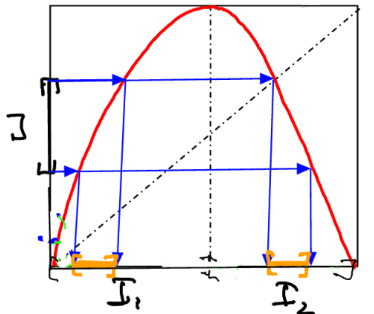
\includegraphics[width=0.4\textwidth]{figures/ch6/24J_preimage.png}
	\caption{The preimage of a subset $J\subset I$, with its closed, nonempty, and connected intersections with $I_1$ and $I_2$.}
	\label{fig:J_preimage}
\end{figure}

\begin{remark}[]
	For any two sets $A$ and $B$ we have that 
	\begin{align}
		f^{-1}(A \cap B) = f^{-1}(A) \cap f^{-1}(B).
	\end{align}
\end{remark}

Further observe that for $I_{s_0s_1}=I_{s_0}\cap f^{-1}(I_{s_1})$ is closed, nonempty, and connected for all $s_0$ and $s_1$ by the previous note. Continuing this we find that
\begin{align}
	I_{s_0s_1s_2} = I_{s_0} \cap f^{-1}(I_{s_1}) \cap f^{-2}(I_{s_2}) = I_{s_0} \cap f^{-1} \left( I_{s_1} \cap f^{-1}(I_{s_2})\right) 
\end{align}
is closed, nonempty, connected, and contained in $I _{s_0s_1}$. This line of argument can be continued to show for any $n \in \mathbb{N}$ the set $I_{s_0\ldots s_n}$ is closed, nonempty, connected, and contained in $I_{s_0 \ldots s_{n-1}}$. Thus we have a nested sequence of closed, nonempty, and connected sets. By Cantor's theorem a nonempty limit exists, which is now not a Cantor set in this case, because it is connected. It is also possible to show that $\lim_{n\to \infty }|I_{s_0 \ldots s_n}| = 0$, where $|\cdot|$ denotes the length of a interval. Now we can can conclude that the limit set contains a single point $x$, therefore as $n\to \infty $ the function $\Psi(s)=x$ is well-defined. It is also true that every element $x\in I$ can be written in this form for some $s$, i.e. $\Psi$ is a surjection.

 Additionally with the metric
 \begin{align}
	 d(s,s') = \sum_{i=0}^{\infty } \frac{|s_i - s'_i|}{2^{i}}	
 \end{align}
the function $\Psi$ is continuous. 

By definition, a single iteration of the map $f$ is equivalent to a shift to the left on the corresponding symbols in $\Sigma$, i.e.
\begin{align}
	f: x= \bm{.} s_0 s_1 s_2 \ldots \mapsto \bm{.} s_1 s_2 \ldots = f(x).
\end{align}
Therefore we have the following commuting diagram
\begin{equation}
\begin{tikzcd}
	\Sigma \arrow[r, "\sigma"] \arrow[d,"\Psi"] 
& \Sigma \arrow[d, "\Psi"] \\
I \arrow[r, "{f}"]
& I 
\end{tikzcd}.
\end{equation}
In comparison to the previous example, $\Psi$ is not invertible (although it is well-defined and continuous). The invertibility of $\Psi $ only fails on a countable set of points $\left \{ f^{-n}\left(\frac{1}{2}\right) \right \}$. Therefore we have that the logistic map is chaotic on $\tilde{I}$.
 \end{ex}

 The previous example leads us to the definition for maps such as the logistic map
\begin{definition}[Topological semi-conjugacy]
	A map $f$ is \emph{topologically semi-conjugate} to $\sigma$ if there exists a surjection $\Psi$ such that
	\begin{align}
		\boxed{
			f \circ \Psi = \Psi \circ \sigma.
		}
	\end{align}
\end{definition}
 
